\documentclass[12pt,Bold,letterpaper,TexShade]{mcgilletdclass}
\usepackage[utf8]{inputenc}
\usepackage{amsmath}
\usepackage{subcaption}
\usepackage{amsfonts}
\usepackage{amssymb}
\usepackage{listings}
    \lstset{basicstyle=\ttfamily\small\color{black}}
\usepackage{mathtools}
\usepackage{mathabx}
\usepackage{graphicx}
\usepackage{braket}
\usepackage{notoccite}
\bibliographystyle{unsrtnat}
\usepackage[sort&compress,numbers]{natbib}
\usepackage{bm}
\usepackage[toc,page]{appendix}
\pagenumbering{arabic}
\usepackage{tikz}
\usetikzlibrary{positioning}
\usetikzlibrary{shapes,arrows}
\pagenumbering{arabic}
\usepackage{algorithm2e}
\usepackage{cleveref}
\usepackage{appendix}
\linespread{1.3}







\SetTitle{\huge{Simulating Optical Pumping\\in the Laser Spectroscopy \\Experiment at TRIUMF}}%
\SetAuthor{Julien Refour}%
\SetDegreeType{Masters of Science}%
\SetDepartment{Department of Physics}%
\SetUniversity{McGill University}%
\SetUniversityAddr{Montreal, Quebec}%
\SetThesisDate{2017-12-14}%
\SetRequirements{Requirements Statement}%
\SetCopyright{Copyright Statement}%



%% Input any special commands below
%\newcommand{\Kron}[1]{\ensuremath{\delta_{K}\left(#1\right)}}
\listfiles%



\tikzstyle{decision} = [ellipse, minimum width=1.5cm, minimum height=1cm, text centered, draw=black, fill=green!30]

\tikzstyle{block} = [rectangle, draw, fill=blue!20, 
    text width=6em, text centered, rounded corners, minimum height=4em]

\tikzstyle{end} = [rectangle, draw, fill=yellow!20, 
    text width=6em, text centered, rounded corners, minimum height=4em]

\tikzstyle{prelim} = [rectangle, draw, fill=red!20, 
    text width=6em, text centered, rounded corners, minimum height=4em]

\tikzstyle{arrow} = [thin,->,>=stealth]





\begin{document}
\citeindextrue
\maketitle
\begin{romanPagenumber}{2}%

%\SetDedicationName{\MakeUppercase{Dedication}}%
%\SetDedicationText{This document is dedicated to the graduate students of the McGill University.}%
%\Dedication

\SetAcknowledgeName{\MakeUppercase{Acknowledgements}}%
\SetAcknowledgeText{In no particular order, I must thank my supervisors: Dr. Matthew Pearson, Dr. Fritz Buchinger and Dr. John Crawford (between the three of which exists a well of endless patience and advice) and Andrea Teigelhoefer, who repeatedly helped me with the theoretical part of this work. Of course, I would like to thank my parents, without whom I may never have had the drive, desire or support to complete this thesis. Finally, thanks must be extended to all the friends that have made Vancouver more of a home than I could ever imagine.}%
\Acknowledge%


%%%%%%%%%%%%%%%%%%%%%%%%%%%%%%%%%%%%%%%%%%%%%%%%%%%%%
%%         English Abstract                        %%
%%%%%%%%%%%%%%%%%%%%%%%%%%%%%%%%%%%%%%%%%%%%%%%%%%%%%
\SetAbstractEnName{\MakeUppercase{Abstract}}%
\SetAbstractEnText{Laser spectroscopy is a technique that can be used to probe the electronic structure of atoms/ions. The Collinear Fast Beam Spectroscopy (CFBS) group at TRIUMF uses this technique to probe the hyperfine structure of rare isotopes produced on-site. The hyperfine structure of an atom, which arises from the various interactions between the atom's/ion's electrons and nucleus, can be used to infer properties, such as the spin and mean squared charge radius, of the atom's nucleus. However, the geometry of the experimental set up at TRIUMF allows for the possibility of optical pumping, a process by which the atoms/ions being probed have their electronic ground state distribution changed before the hyperfine structure can be measured. This in turn can change the relative intensities of the hyperfine transitions being measured. Optical pumping depends, mainly, on the power of the laser used to excite the hyperfine transitions being studied. In this work, a statistical model designed to simulate the effects of optical pumping on hyperfine spectra measured at TRIUMFs CFBS experiment. With the goal of simulating the hyperfine spectrum of any atom under investigation, the model is based on the likelihood that an atom/ion reaches the region where the hyperfine spectrum is measured in its original ground state. This likelihood is in turn used the modify the relative intensities of each hyperfine transition. The effects of laser power, the temperature of the atoms/ions, and the distance they must travel before being measured are examined. Additionally, the predictions of the model are compared to previously measured Gallium-69 and Rubidium-87 hyperfine spectra. Discrepancies between the assumed temperature and the temperature predicted by the model were observed in the case of Gallium-69, with a possible resolution being the effects of accelerating the atoms/ions when they are extracted from a Radio Frequency Quadrupole trap used for bunching. In the case of Rubidium-87, a discrepancy between the expected and measured relative intensity of particular transition is observed. This may be due to an over-estimation of the power delivered to the atoms.}
\AbstractEn%

%%%%%%%%%%%%%%%%%%%%%%%%%%%%%%%%%%%%%%%%%%%%%%%%%%%%%
%%         French Abstract                         %%
%%%%%%%%%%%%%%%%%%%%%%%%%%%%%%%%%%%%%%%%%%%%%%%%%%%%%
\SetAbstractFrName{\MakeUppercase{ABR\'{E}G\'{E}}}%
\SetAbstractFrText{Un model statistique, construit pour la simulation des effets du pompage optique sur les spectres hyperfines mesurés à TRIUMF, est présenté. Les résultats de ce model, construit sur la probabilité qu’une atome arrive dans la région d’interaction dans son état de repos original, sont comparés avec des spectres mesurés du Gallium-69 et Rubidium-87. Dans le cas du Gallium-69, une différence entre la température assumée et la température calculée a été observée, provenant peut-être des effets des voltages appliqués aux atomes lors de leur extraction et accélération. Pour le Rubidium-87, une différence entre les intensités mesurée et calculés de la transition $F_e = 1 \rightarrow F_g = 2$ a été observée, les origines de laquelle viennent d’une surestimation de l’intensité du laser.}%
\AbstractFr%

\TOCHeading{\MakeUppercase{Table of Contents}}%
\LOTHeading{\MakeUppercase{List of Tables}}%
\LOFHeading{\MakeUppercase{List of Figures}}%
\tableofcontents %
\listoftables %
\listoffigures %

\end{romanPagenumber}
%\mainmatter %
 
\chapter{Introduction}
\label{Intro}
\noindent First observed in 1892 \citep{michelson}, the splitting of the spectral line of a single atomic transition, now known as the hyperfine splitting or structure of a transition, was theoretically described in 1924 by Wolfgang Pauli\citep{Pauli1924}. The development of quantum mechanics allowed Pauli to propose that the hyperfine splitting of a transition arose from the interaction of the orbital electrons and a small nuclear magnetic moment. In 1931, H. Schüler and T. Schmidt proposed the additional contribution of a nuclear electric quadrupole moment to the hyperfine splitting, completing the modern understanding of the interaction mechanisms\citep{Lieb2001}.

The existence of hyperfine structure offers the unique opportunity to study the structure of the nucleus of an atom by probing the structure of a particular electronic transition. The nuclear magnetic moment proposed by Pauli depends on the spin of the nucleus, while the electric quadrupole moment described by Schüler and Schmidt depends on the distribution of charge in the nucleus. If the nuclear spin and the angular momentum state of the electron in both the ground and excited states are known, then the expected hyperfine structure can be determined by up to four parameters. Known as the hyperfine coefficients, these parameters describe the strength of the electron-nucleus interactions that give rise to the hyperfine structure. If the hyperfine spectrum of a transition can be measured empirically, the hyperfine coefficients and, by consequence, the nuclear structure can be determined. 

Laser spectroscopy is a technique through which the hyperfine spectrum of a transition can be measured. Briefly, atoms (or ions) are exposed to laser radiation. The frequency of this radiation is scanned such that, in the rest frame of the atom/ion, it comes into resonance with an allowed atomic transition. For reasons of efficiency when working with radioactive beams, the collinear geometry is used. The laser frequency is scanned by Doppler shifting the atoms/ions into resonance, rather than changing the frequency of the laser itself. Through the adjustment of their velocity, the atoms/ions can be moved in to and out of resonance with a chosen transition. Resonant velocities (and thus energies) will excite electrons through a hyperfine transition. The subsequent de-excitation of these electrons produces an excess of photons that can be measured using a set of light collection instruments. The location of these peaks with respect to each other determine the values of the hyperfine parameters and, in turn, the nuclear structure. 

As with all experimental techniques, laser spectroscopy has its drawbacks. Among others, an effect known as optical pumping can severely change the outcome of a measurement. Optical pumping occurs when the atoms are exposed to the laser for a significant time before passing through the light collection region. This prolonged exposure to the laser can change the ground state distribution of the atoms, which in turn can cause certain hyperfine peaks to be drowned out or emphasized, altering the results of the ensuing hyperfine coefficient calculations. The strength of optical pumping depends on the isotope being investigated, the power of the exciting laser as well as the overall geometry of the experimental set up.

This work develops a procedure through which the effects of optical pumping on a given hyperfine spectrum can be simulated. In particular, this work focuses on the laser spectroscopy experiment set up at TRIUMF, Canada's national nuclear physics laboratory. The following Chapter briefly outlines TRIUMF's general structure, as well as how laser spectroscopy is done on site. Chapter 3 provides a theoretical background to the mechanisms that lead to hyperfine splitting, while chapter 4 describes and demonstrates the effects of optical pumping on a hyperfine spectrum. The methods used to simulate the effects of optical pumping at TRIUMF are also presented in this section, with the results presented in Chapter 5. A summary and some concluding remarks are given in Chapter 6, and, finally, the developed program is found in the appendix. 

\chapter{Laser Spectroscopy at TRIUMF}
\label{Lspec}
\input{Laser_spec_triumf/laser_spec_triumf.tex}

\chapter{Theory of Laser Spectroscopy}
\label{theory}
\noindent In this chapter, the theoretical background necessary to the understanding and simulation of a hyperfine spectrum is presented. $\S$ \ref{AHF} describes how the features of a hyperfine spectrum are linked to the physical properties of a nucleus, while $\S$ \ref{ALI} outlines the way in which lasers interact with atoms.
Note: Throughout this section, a variable written in a bold typeface is vector valued, while its non-bold counterpart is its magnitude. 
\section{Anatomy of a Hyperfine Spectrum}
\label{AHF}
\begin{figure}[h]
\includegraphics[width=\textwidth]{Graphics/spec_with_peaks_4.png}
\caption[Hyperfine spectrum and level-scheme for Gallium-69.]{Hyperfine spectrum and level-scheme for the 4P$_{3/2}\rightarrow$5S$_{1/2}$ transition in atomic Gallium-69. Photon counts are shown on the vertical axis, while the horizontal shows the energies of the photons. Each allowed transition in the level-scheme is linked to the relevant peak in the hyperfine spectrum.}
\label{ga69}
\end{figure}
How can the properties of a hyperfine spectrum, such as that of $^{69}\mathrm{Ga}$ shown in Fig. \ref{ga69}, be translated into measurements of the physical properties of the nucleus? The hyperfine spectrum is, after all, the result of probing the electronic structure of the atom. The answer is that the electrons interact with the nucleus through several mechanisms, each of which will be described in this section. To begin, however, consider the following system: An electron transitions from a ground state $\ket{g}$ to an excited state $\ket{e}$. More precisely $\ket{g}$ and $\ket{e}$ are defined as 
\begin{align}
\ket{g} =& \ket{n_g,\mathrm{\bf{J}_g,J_{g,z}}}\\
\ket{e} =& \ket{n_e,\mathrm{\bf{J}_e,J_{e,z}}},
\end{align}
where $n_{g,e}$ are principal quantum numbers, and $\bf{J}_{g,e}=\bf{L}_{g,e}+S$ and $\bf{J}_{g,e}^z$ are the angular momentum and projection of the angular momentum on an axis of quantization $z$, respectively. $\bf{L}$ is the orbital angular momentum and $\bf{S}$ the spin of the electron. Next, if nucleus of the atom in which this transition is occurring has angular momentum $\bf{I}$, then a new vector, $\bf{F}$, can be defined as 

\begin{equation}
\bf{F_{g,e}} = \bf{I} + \bf{J}_{g,e}
\end{equation}
$\bf{F}$ describes the total angular momentum state of the atom, so $\ket{g}$ and $\ket{e}$ can be rewritten as

\begin{align}
\ket{g} =& \ket{n_g,\mathrm{F_g, F_{g,z}}}\\
\ket{e} =& \ket{n_e,\mathrm{F_e, F_{e,z}}}
\end{align}
For a fixed I, F can range from $(|\mathrm{I-J}|)$ to $(|\mathrm{I+J}|)$.
\subsection{Peak Energies}
The energy of the electrons depends on the various electron-nucleus interactions present in the atom. For the purposes of this work, only three interactions are considered. These are the isotope, magnetic dipole and electric quadrupole shifts, which lead to energy shifts on the order of roughly $10^{-7}-10^{-4}$ eV\cite{ModAN}. There are higher order interactions (magnetic octopole, electric hexadecapole), however their effects are far below the resolution of $\approx 10^{-8}$ eV of the experimental set-up employed at TRIUMF\cite{GA69}.

\subsubsection{Isotope Shift}
The isotope shift is measured with respect to a reference isotope. As neutrons are added or removed from a nucleus, the charge distribution, as well as the mass, of the nucleus changes. This leads to three different effects on the energies of the electrons. 

The change in the mass of the nucleus leads to what is known as the Mass Shift, $\Delta E_M$. The Mass Shift between two isotopes with mass numbers A and A' is given by\citep{TomT}
\begin{equation}
\Delta E_M = \frac{m_{\mathrm{A}}-m_{\mathrm{A'}}}{2 m_{\mathrm{A}} m_{\mathrm{A'}}} \left(\sum_i\mathrm{\textbf{p}}_i +2 \sum_{i>j}\mathrm{\textbf{p}}_i \cdot \mathrm{\textbf{p}}_j \right),
\end{equation}
where $m_{\mathrm{A}}$ and $m_{\mathrm{A'}}$ are the isotope masses, and $\textbf{p}_i$ is the momentum of the i$^{\mathrm{th}}$ election. The first term is the Bohr reduced mass equation arising from the change in the center of mass of the system, while the second term takes into account the correlations between the momenta of all the electrons. 

The change in the charge distribution of the nucleus produces the Field Shift. While the typical nucleus is far smaller the wavefunction of a typical orbital electron, the effect is still important. The energy of a nucleus in the charge density produced by the electrons at the origin, $E_F$, is given by

\begin{equation}
E_F = \frac{Ze^2}{6 \epsilon_0}|\psi(0)|^2 \left\langle r_{ch}^2\right\rangle
\end{equation}
where $\epsilon_0$ is the permitivity of free space, $Z$ is the proton number, $e$ is the fundamental charge, $\psi(0)$ is the value of the electron wavefunction at the nucleus. $ \left\langle r_{ch}^2\right\rangle$ is the mean-square charge radius of the nucleus, defined as \cite{LasCool}
\begin{equation}
 \left\langle r_{ch}^2\right\rangle = \frac{\int_0^{\infty}\rho(\mathbf{r})r^2dV}{\int_0^{\infty}\rho(\mathbf{r})dV}.
\end{equation}
\noindent The Field Shift between two isotopes is then given by
\begin{equation}
\Delta E_F =  \frac{Ze^2}{6 \epsilon_0}\Delta|\psi(0)|^2 \Delta\left\langle r_{ch}^2\right\rangle
\end{equation}

\noindent In total, then, the isotope shift $\Delta E_{\mathrm{A,A}'}$ is given by
\begin{equation}
 \Delta E_{\mathrm{A,A'}} = \Delta E_M + \Delta E_F
\end{equation}
\noindent Typically, $\Delta E_M$ can be calculated beforehand. $ \Delta E_F$, however, must be determined experimentally, due to the difficulties associated with calculating $\Delta|\psi(0)|^2$.
\noindent \subsubsection{Magnetic Dipole Interaction}
A nucleus with a non-zero nuclear spin $\bf{I}$  will have a magnetic dipole moment, given by

\begin{equation}
\boldsymbol{\mu}_{\mathrm{\bf{I}}} = g_{\mathrm{I}}\mu_{\mathrm{N}}\mathrm{\bf{I}}
\end{equation}

\noindent where $g_{\mathrm{I}}$ is the g-factor and $\mu_{\mathrm{N}}$ is the nuclear magneton\cite{Nut}. The interaction of $\mu_{\mathrm{I}}$ with the magnetic field produced by the electrons, $\mathrm{\bf{B_e}}$, creates a shift in the energy of the orbiting electrons. Provided the electrons occupy an angular momentum state $\mathrm{\bf{J}} \neq 0$ (since $\mathrm{\bf{J}} = 0 \rightarrow \mathrm{\bf{B_e}} = 0$), the Hamiltonian for this interaction is given by \cite{TomT}

\begin{equation}
\mathcal{H} = -\boldsymbol{\mu}_{\mathrm{\bf{I}}} \cdot \mathrm{\bf{B_e}}
\end{equation}

\noindent This interaction leads to a shift, $\Delta E_{\mu_I}$, in the energy of the atomic states by

\begin{equation}
\Delta E_{\mu_I} = \frac{AK}{2}
\end{equation}
where $K = \mathrm{F(F+1) - I(I+1) - J(J+1)}$ and 

\begin{equation}
A = \frac{\mu_{\mathrm{I}}\mathrm{B_e}}{\mathrm{IJ}}
\end{equation}

\noindent \subsubsection{Electric Quadrupole Interaction}
The electric quadrupole moment is used to describe the distribution of charge in a nucleus. For a nucleus composed of $n$ protons and $\mathbf{I}\geq1$, the electric quadrupole moment, Q, is given by

\begin{equation}
\mathrm{Q} = \sum_i^n (3z_i^2-r_i^2)
\end{equation}
where $r_i^2 = x_i^2+y_i^2+z_i^2$ for a chosen $z$-axis\cite{Nut}. Noting that the deformations described by Q are defined with respect to the $z-$axis, Fig. \ref{Q} shows how different values of Q translate into physical differences in the charge distribution of the nucleus. If Q $ < 0$, then the nucleus is stretched in the $x-y$ plane (oblate). If Q $ > 0$, then the nucleus is stretched along the $z-$axis (prolate). Q $=0$ indicates that the nucleus is spherical. 

\begin{figure}[h]
\begin{center}
\includegraphics[width=\textwidth]{Graphics/Q_pic.png}
\caption[Oblate vs. Prolate vs. Spherical]{\small Shape of the nucleus for Q $<$ 0 (oblate), Q $>$ 0 (prolate) and Q $=$ 0 (spherical)\cite{wolf}.}
\label{Q}
\end{center}
\end{figure}

In reality, direct measurement of Q is not feasible, as the nucleus is rotating. Instead, the spectroscopic quadrupole, Q$_s$, is measured. Q$_s$ is defined as the projection of Q onto the axis of quantization of the nucleus, and is given by
\begin{equation}
\mathrm{Q}_s = \frac{\mathrm{I}(2\mathrm{I}-1)}{(\mathrm{I}+1)(2\mathrm{I}+3)}\mathrm{Q},
\end{equation}
The use of $Q_s$ as a measure of $Q$ is valid under the assumption that the nuclear deformation is axially symmetric. Additionally, it is assumed that the axis of symmetry has a well defined direction with respect to \textbf{I}.

The Hamiltonian for the interaction between the spectroscopic electric quadrupole moment and the electric field produced by the electrons at the nucleus, $E_N$, is given by

\begin{equation}
\mathcal{H} = - \frac{1}{6}e\mathrm{Q}_s\nabla{E_N}
\end{equation}
where
\begin{equation}
\nabla{E_N} = \frac{\partial^2V}{\partial x_i\partial x_j}, \{x_j,x_k\} \in \{x,y,z\} \otimes \{x,y,z\},
\end{equation}
$e$ is the fundamental charge and $V$ is the electric potential\cite{TomT}. Recalling that the nuclear deformation is symmetric about the axis of quantization, the shift in energy is then given by

\begin{equation}
\Delta E_{\mathrm{Q_s}} = \frac{B}{4}\left[\frac{\frac{3}{2}K(K+1)-2\mathrm{I}(\mathrm{I}+1)\mathrm{J}(\mathrm{J}+1)}{\mathrm{I}(2\mathrm{I}-1)\mathrm{J}(2\mathrm{J}-1)}\right]
\label{B-eq}
\end{equation}
where $B$ is a hyperfine coefficient and is given by \cite{TomT}
\begin{equation}
B = e\mathrm{Q_s}\left\langle\frac{\partial^2V}{\partial z^2} \right\rangle.
\end{equation}
Eq. \ref{B-eq} has singularities at I = $\frac{1}{2}$ and J=$\frac{1}{2}$. This captures the fact that in either case there is no coupling between the nucleus and the electric field gradient produced by the electrons, as an orbital angular momentum state of $\frac{1}{2}$ is isotropically distributed in space .

\subsubsection{The Hyperfine Equation}
The resonant energy of a transition between $\ket{g}=\ket{n_g,\mathrm{\textbf{F}_g=\textbf{I} + \textbf{J}_g}}$ and $\ket{e}=\ket{n_e,\mathrm{\textbf{F}_e=\textbf{I} + \textbf{J}_e}}$ is then given by
\begin{equation}
E_{hfs} = E_{fs} +  \Delta E_{\mathrm{A,A'}}+\Delta E_{\mu_I}\Bigr|_{\mathrm{F_g},I,J_g}^{\mathrm{F_e},I,J_e}+\Delta E_{\mathrm{Q_s}}\Bigr|_{\mathrm{F_g},I,J_g}^{\mathrm{F_e},I,J_e}.
\label{HFE}
\end{equation}

\noindent When a hyperfine spectrum is fitted, the fit parameters which govern the locations of the peaks are the hyperfine parameters $A$ and $B$ for both $\ket{e}$ and $\ket{g}$, as well as what is known as the centroid, $\nu_0$. The centroid combines the fine structure energy and the isotope shift into one quantity. It is important to note that while the values of hyperfine coefficients can be directly linked to the physical properties of the nucleus, only the change in the centroid with respect to a reference isotope can be used to measure the change in the mean-square charge radius.

\subsection{Peak intensities} 
The other notable characteristic of a hyperfine spectrum, the ratios of the peak intensities can give information as to the spin of the nucleus if the angular momentum states of the electron orbitals are known. The origin of the peak intensities is presented in more detail in the Angular Part of $\S$ \ref{ALI}, however in the interest of the completeness of this section, the result is presented here. The intensity of a transition from $\ket{\mathrm{\bf{F}_e,\bf{J}_e,I}}$ to $\ket{\mathrm{\bf{F}_g,\bf{J}_g,I}}$, relative to other available transitions, is known as the Racah intensity and is given by
\begin{equation}
Intensity = (2\mathrm{F}_e+1)(2\mathrm{F}_g+1)
\left\lbrace
\mathrm{
\begin{matrix}
\mathrm{F_g} & \mathrm{F_e} & 1\\
\mathrm{J_e} & \mathrm{J_g} & \mathrm{I} 
\end{matrix}
}
\right\rbrace^2
\label{RACAH}
\end{equation}
where the quantity in curly brackets is the Wigner 6-j symbol\cite{TomT}. An important property of the Racah intensities is the dependence on I. In cases where the value of I may be ambiguous, the relative intensities of the transitions can be used to discriminate between values of I.
\subsection{Peak Widths}
The lineshape of the peaks is the result of three physical processes, outlined in this section. These three processes are of varying importance, depending on the properties of the atoms being probed, contributing Lorentzian or Gaussian profiles to the peak shape. 

\subsubsection{Natural Linewidth}
The first addition to the linewidth of an atomic transition is the natural linewidth. The energy-time version of the uncertainty principal, $\Delta E \Delta t= \hbar$ leads to 
\begin{equation}
\Delta \nu = \frac{\Delta E}{h}=\frac{1}{2 \pi \tau_0}
\end{equation}
where $\tau_0$ is the mean lifetime of the state and $\Delta \nu$ is the full width half maximum of the Lorentzian profile describing the natural lineshape of an atomic transition\cite{TomT}.

\noindent \subsubsection{Power Broadening}
Stimulated emission occurs when an atom in an excited state is in the presence of photons with energy similar to an available atomic transition. In the case of laser spectroscopy, the laser provides the source of stimulating photons. Stimulated emission leads to power broadening, which depends on the power of the laser. The lifetime of a state will decrease according to
\begin{equation}
\frac{1}{\tau}= \frac{1}{\tau_0}\sqrt{1+\frac{I}{I_s}},
\end{equation}
where $I$ is the laser intensity and $I_s$ is the saturating laser intensity, which occurs when the rate of absorption is equal to the rate of stimulated emission on resonance. The expected lifetime of an excited electron decreases, resulting in a Lorentzian contribution to the lineshape as a consequence of the energy-time version of the uncertainty principal\cite{TomT}.
\subsubsection{Doppler Broadening}
Doppler broadening occurs when the atoms have a thermal velocity spread along the direction of propagation. This velocity spread leads to a shift in the frequency of the laser observed as by the atoms. The velocity distribution of a collection of atoms with mass $m_A$ at temperature $T$, along an axis $z$, is given by the so-called Maxwell-Boltzmann distribution \cite{thermal}
\begin{equation}
P(v_z) = \sqrt{\frac{m_A}{2 \pi kT}}\exp\left(-\frac{m_Av_z^2}{2kT}\right)
\label{MBD}
\end{equation}
\noindent where $k$ is the Boltzmann constant and $v_z$ is the velocity component of the atoms along the $z$-axis. The half width half maximum (HWHM) of this distribution is
\begin{equation}
\mathrm{HWHM} = \sqrt{\frac{2\log{(2)}kT}{m_A}}.
\end{equation}
For a Gaussian lineshape, the HWHM is also give by
\begin{equation}
\mathrm{HWHM} = \sqrt{2\log(2)}\sigma_g
\end{equation}
where $\sigma_g$ the square root of the variance of the distribution, $\sigma_g^2 = kT/m_A$ in the case of a Gaussian profile. When an observer is moving relative to a source of radiation, the frequency of the radiation measured by the observer obeys the following \cite{landau1975}
\begin{equation}
f_o = f_s\sqrt{\frac{1+v/c}{1-v/c}}
\label{dop_shift}
\end{equation}
where $f_o$ and $f_s$ are the observed and source frequencies, respectively, $v$ is the velocity of the observer relative to the source and $c$ is the speed of light in a vacuum. Differentiating the above with respect to $v$, and assuming $v\ll c$ leads to
\begin{align*}
\frac{df_o}{dv} =& 2\frac{f_s}{c}\\ \nonumber
df_o =& f_s\left(\frac{8kT\log(2)}{m_Ac^2}\right)^{1/2}
\end{align*}
\label{temp_width}
$df_o$ is the HWHM of the Gaussian lineshape that Doppler broadening contributes to the overall lineshape of the transition\cite{TomT}.

\subsubsection{Voigt Profile}
As the strengths of the above processes can change depending on the parameters of the experiment, a Voigt profile is used when fitting the hyperfine spectra. The Voigt profile, defined as a convolution of the Lorentzian and Gaussian profiles, has no exact analytic solution. For the purposes of this work, the Pseudo-Voigt profile, given below, is used.
\begin{equation}
\mathcal{V}(x) = \frac{1-\epsilon}{\sigma_g\sqrt{2\pi}}\exp\left(\frac{(x-x_0)^2}{2\sigma_g^2}\right)+\frac{\epsilon\sigma}{\pi((x-x_0)^2+\sigma^2)}
\end{equation}
This is the weighted sum of a Gaussian and a Lorentzian where $\epsilon$ is a parameter that determines the relative contribution of the each and $x_0$ is the centroid. $\sigma$ is the Voigt linewidth and $\sigma_g = \sigma/\sqrt{2\log{2}}$ is defined such that the full width half maximum of the profile as well as its components is $2\sigma$\cite{voigt}.
\section{Spontaneous Emission in \\ Multi-Level Atoms}
\label{ALI}
A hyperfine spectrum is constructed through the measurement of the photons emitted as electrons in excited states de-excite to lower energy states. In order to simulate a hyperfine spectrum, then, it is necessary to understand the mechanisms through which electrons transition between energy levels in an atom.

Consider a two-level atom in an excited state. The wavefunction of the system is given by
\begin{equation}
\ket{\psi} = c_{e,0}e^{-i\omega_et}\ket{e,0} + \sum_Sc_{g,1}e^{-i(\omega_g+\omega)t}\ket{g,1_S}
\end{equation}
where $S = (\bm{k},\bm{\varepsilon})$ gives the wavevector $\bm{k}$ and polarization $\bm{\varepsilon}$ of an emitted photon, $\omega = kc$, $\omega_e$ and $\omega_g$ are the angular frequencies corresponding to the energy of the excited and ground states, respectively\cite{LasCool}. The time evolution of the two states is described by
\begin{align}
i\frac{\mathrm{d}c_{e,0}(t)}{\mathrm{d}t} =& \sum_Sc_{g,1_S}(t)\Omega_S e^{-i(\omega-\omega_a)t} \label{dc_e} \\
i\frac{\mathrm{d}c_{g,1_S}(t)}{\mathrm{d}t} =& \ c_{e,0}(t)\Omega_S^*e^{i(\omega-\omega_a)t} \label{dc_g}
\end{align}
where the coupling between each state is given by the Rabi frequency \\$\Omega_s = -\bm{\mu}\cdot\bm{E}_{\omega}/\hbar$. The electric dipole moment, $\bm{\mu}$ between two states is given by
\begin{equation}
\bm{\mu} = e\bra{e}\bm{r}\ket{g} 
\end{equation}
and the electric field per mode is given by
\begin{equation}
\bm{E}_{\omega} = \sqrt{\frac{\hbar\omega}{2\epsilon_0V}}\bm{\varepsilon}.
\end{equation}
$V$ is the volume over which the field is quantized and will eventually drop out. Integration of Eq. \ref{dc_g} and substitution of the result into Eq. \ref{dc_e}, followed by further integration yields 
\begin{equation}
\frac{d c_{e,0}(t)}{dt} = -\frac{\gamma}{2}c_{e,0}(t),
\end{equation}
where
\begin{equation}
\gamma = \frac{\omega^3\mu^2}{3\pi\epsilon_0\hbar c^3}
\label{gamma}
\end{equation}
is the decay rate for the population of the excited state, $\omega$ is the frequency of the transition and $c$ is the speed of light in a vacuum. The mean lifetime of the excited state is given by $\tau = 1/\gamma$. For an excited state where multiple decay paths are available, the total decay rate, $\gamma_t$ is given by
\begin{equation}
\frac{1}{\gamma_t} = \sum_i \frac{1}{\gamma_i}
\label{totdec}
\end{equation}
where the $\gamma_i$ are the partial decay rates for each decay path.


\subsection{The Dipole Moment}
In general, calculating the dipole moment  $\mu = \bra{e} \bm{\varepsilon} \cdot \bm{r} \ket{g}$ is not a simple task. 
In the simplest case (read hydrogenic wavefunctions), the Wigner-Eckart theorem states that the dipole moment can be split into two separate quantities in the following manner \citep{LasCool}
\begin{equation}
\mu_{eg} = e \mathcal{R}_{n_e J_e, n_g J_g}\mathcal{A}_{J_eJ_e^z, J_gJ_g^z}
\label{muref}
\end{equation}
where $\mathcal{R}_{n_e J_e, n_g J_g}$ and $\mathcal{A}_{J_eJ_e^z, J_gJ_g^z}$ are the radial and angular parts of the dipole moment, described in more detail below. 
\subsubsection*{Radial Part}
In most cases where the hyperfine structure is being probed, the radial part of the dipole moment only acts as an overall multiplicative factor for the strength of the coupling between the excited and ground states. This is due to the fact that all available ground states typically share the same radial wavefunction, likewise in the case of the excited states. The radial part is given by
\begin{equation}
\mathcal{R}_{n_e J_e, n_g J_g} = \bra{R_{n_e J_e}}\bm{r}\ket{R_{n_g J_g}} = \int_0^{\infty}r^2R_{n_e J_e}(r)rR_{n_g J_g}(r)dr
\end{equation}
where the $R_{nJ}$ are the hydrogenic radial wavefunctions of their respective states
\begin{equation}
R_{nJ}(r) = N_{nJ}\rho^J\exp(-\rho/2)J_{n-J-1}^{2J+1}(\rho)
\end{equation}
where $N_{nJ}$ is a normalization constant and $J_{n-J-1}^{2J+1}(\rho)$ are the Laguerre polynomials evaluated at $\rho = 2r/na_0$, where $a_0$ is the Bohr radius. The $J_{n-J-1}^{2J+1}(\rho)$ can be expanded in a power series
\begin{equation}
J_{n}^{m}(r) = \sum_{k=0}^{n} c_kr^k
\end{equation}

It is possible to extend this analysis to atomic structures that have an isolated electron sitting outside a closed shell. This is done using the effective principal quantum number $n^*= n - \delta_{J}$, where $\delta_{J}$ is called the quantum defect and depends on the orbital angular momentum \textbf{J}. This extended analysis is, however, not necessary, as an empirical measure of $ \mathcal{R}^2_{n_e J_e, n_g J_g}$ is easily obtained, and remains constant over all hyperfine transitions. This is done through the use of the decay rate of the fine-structure transition, $\gamma_f$. From Eq. \ref{totdec}, the decay rate of the fine-structure excited state is given by
\begin{equation}
\frac{1}{\gamma_f} = 3 \pi \epsilon_0 \hbar c^3 \sum_i \frac{1}{\omega_i^3 \mu_i^2}
\end{equation}
Substitution of Eq. \ref{muref} in to the above yields
\begin{equation}
\frac{1}{\gamma_f} = \frac{3 \pi \epsilon_0 \hbar c^3}{\mathcal{R}^2e^2} \sum_i \frac{1}{\omega_i^3\mathcal{A}^2_i}
\end{equation}
where the subscripts on $\mathcal{R}$ and $\mathcal{A}$ have been dropped for convenience. Rearranging gives the following expression for $\mathcal{R}^2$
\begin{equation}
\mathcal{R}^2 = \frac{3 \pi \epsilon_0 \hbar c^3 \gamma_f}{e^2} \sum_i \frac{1}{\omega_i^3\mathcal{A}^2_i}.
\label{Remp}
\end{equation}
Note that this result allows $\mathcal{R}$ to take both negative and positive values. For the purposes of the calculations present in this work, however, only the square of the radial part is important. As such, the degeneracy in Eq. \ref{Remp} can safely be ignored. 
\subsubsection*{Angular Part}
Unlike the radial part of the dipole moment, the angular part changes depending on the F state of the excited and ground states. An outline of the procedure followed to find $\mathcal{A}$ is outlined in this section, a complete treatment of the calculation can be found in \cite{LasCool}. 

In the presence of hyperfine structure, the atomic eigenstates can be represented in the following manner
\begin{equation}
\ket{n,\mathrm{\bf{F}},\mathrm{\bf{F}}_z} = \sum_iC_i\ket{n,\mathrm{\bf{J}},\mathrm{\bf{J}}_z}\ket{\mathrm{\bf{I}},\mathrm{\bf{I}}_z}
\label{jstates}
\end{equation}
where \textbf{J}  =\textbf{ J} + \textbf{S}, \textbf{S} is the spin of the electron and the $C_i$'s are Clebsch-Gordan coefficients. The \textbf{J} states can further be decomposed into combinations of \textbf{J} and \textbf{S} states
\begin{equation}
\ket{n,\mathrm{\bf{F}},\mathrm{\bf{F}}_z} = \sum_iC_i\ket{\mathrm{\bf{I}},\mathrm{\bf{I}}_z}\sum_kC_k\ket{n,\mathrm{\bf{J}},\mathrm{\bf{J}}_z}\ket{\mathrm{\bf{S}},\mathrm{\bf{S}}_z}
\label{jstates}
\end{equation}
This is possible since the optical electric field only couples the orbital angular momentum, \textbf{J}, components of the eigenstates. The Clebsch-Gordan coefficients can be expressed as
\begin{equation}
C_i = \braket{\mathrm{\bf{J},\bf{J}_z ; \bf{S},\bf{S}_z}|\mathrm{\bf{J},\bf{J}_z}}=(-1)^{\mathrm{-J+S-J_z}}\sqrt{\mathrm{2J+1}}
\left(
\begin{matrix}
\mathrm{J}-\mathrm{S} & \mathrm{S} & \mathrm{J}\\
\mathrm{J}_z-\mathrm{S} & \mathrm{S}_z & -\mathrm{J}_z
\end{matrix}
\right)
\end{equation}
where the quantity in brackets is the Wigner 3-j symbol. Substituting Eq. \ref{jstates} into the definition of $\mu$ gives 
\begin{equation}
\begin{split}
\mu = \sum_{q = -1,0,1} e (-1)^{\mathrm{1+J_e+J_g+I-F_{e,z}}}\mathcal{R}_{n_e J_e, n_g J_g}\\
\times \sqrt{(2\mathrm{J}_g+1)(2\mathrm{J}_e+1)(2\mathrm{F}_g+1)(2\mathrm{F}_e+1)}\\
\times \left\lbrace
\begin{matrix}
\mathrm{J}_e-\mathrm{S} & \mathrm{J}_e & \mathrm{S}\\
\mathrm{J}_g & \mathrm{L}_g-\mathrm{S} & 1
\end{matrix}
\right\rbrace
\left\lbrace
\begin{matrix}
\mathrm{J}_e & \mathrm{F}_e & \mathrm{I}\\
\mathrm{F} & \mathrm{J}_g &1
\end{matrix}
\right\rbrace
\left(
\begin{matrix}
\mathrm{F}_g & 1 & \mathrm{F}_e\\
\mathrm{F}_{g,z} & q &-\mathrm{F}_{e,z}
\end{matrix}
\right)
\end{split}
\end{equation}
where the quantity in the curly brackets is not a 3-j symbol but a 6-j symbol, and $q$ is the polarization of the electric field (1,0,-1). Recalling that $\mathcal{R}_{n_e J_e, n_g J_g}$ is a multiplying factor only and can be pulled out of the summation, then the angular part of $\mu$ (Eq. \ref{muref}) is given by
\begin{equation}
\begin{split}
\mathcal{A} = \sum_{q = -1,0,1} e (-1)^{\mathrm{1+J_e+J_g+I-F_{e,z}}}
\times \sqrt{(2J_g+1)(2J_e+1)(2F_g+1)(2F_e+1)}\\
\times \left\lbrace
\begin{matrix}
\mathrm{J}_e-\mathrm{S} & \mathrm{J}_e & \mathrm{S}\\
\mathrm{J}_g & \mathrm{J}_g-\mathrm{S}& 1
\end{matrix}
\right\rbrace
\left\lbrace
\begin{matrix}
\mathrm{J}_e & \mathrm{F}_e & \mathrm{I}\\
\mathrm{F} & \mathrm{J}_g &1
\end{matrix}
\right\rbrace
\left(
\begin{matrix}
\mathrm{F}_g & 1 & \mathrm{F}_e\\
\mathrm{F}_{g,z} & q &-\mathrm{F}_{e,z}
\end{matrix}
\right)
\end{split}.
\end{equation}


\subsection{Selection Rules}
The coupling of the ground state and excited state through the optical electrical field places restrictions on the change in the angular momentum state of the atom. In the case of transitions between orbital angular momentum states present in hyperfine atomic structures, only transitions where $\Delta$\textbf{F}  $=\pm1,0$ are permitted. These selection rules reflect conservation of angular momentum. Photons have angular momentum $\hbar$. The angular momentum of the photon can either be parallel, anti-parallel or perpendicular to the axis of quantization, reflecting $\Delta$\textbf{F}$=\pm1,0$ respectively. Additionally, the transition \textbf{F}' = 0 $\rightarrow$ \textbf{F} = 0 is forbidden. This is because \textbf{F} is a result of the coupling between \textbf{I} and \textbf{J}. \textbf{F}' = 0 implies that \textbf{I} = 0 = \textbf{J}' or |\textbf{I}| = |\textbf{J}|. The emission of a photon requires a change in angular momentum, which is impossible in both cases, as \textbf{J} does not change\cite{TomT}.

\section{Photon Scattering Rates}
The rate at which photons are absorbed by atoms is an important factor in the simulation of hyperfine spectra. For a two level system, where the population of the the excited state $\rho_{e}$ and the ground state $\rho_{g}$ obey the conservation rule $\rho_e +\rho_g = 1$, the total scattering rate from a laser field is given by
\begin{equation}
\gamma_p =  \frac{s_0/2}{1+s_0+(2\delta/\gamma)^2}
\label{scatt_rate}
\end{equation}
where $s_0$ is the on resonance saturation parameter $s_0 = I_l/I_s$, $\delta$ is the detuning parameter and $\gamma$ is the decay rate of the excited state. $I_l$ is the intensity of the laser field and $I_s$ is the saturation intensity defined as
\begin{equation}
I_s \equiv \frac{\pi h c}{3 \lambda^3 \tau}
\end{equation}
where $\lambda$ is the wavelength of emission of a resonant photon and $\tau = 1/\gamma$ is the lifetime of the excited state. The detuning parameter can be defined as
\begin{equation}
\delta =|f_{l} - f_{res}|
\end{equation}
where $f_l$ is the frequency of the laser and $f_{res}$ is the resonant frequency of the transition\cite{LasCool}. Eq. \ref{scatt_rate} provides an easy evaluation of the expected time for an on-resonance photon to be absorbed, which will be needed in the next chapter.



\chapter{Simulation of Optical Pumping}
\label{Op_pump}
\noindent As mentioned in the Chapter \ref{Lspec}, the distance between the CEC and the LCR introduces the possibility of optical pumping, a process that changes the ground state distribution of the atoms as they travel the distance between the two regions. This change in ground state distribution is induced by the interaction of the atoms with the laser before they reach the LCR. In an atomic system that has not interacted with a laser, the ground state distribution of the hyperfine levels is statistical.\cite{townsend} The likelihood of an electron occupying hyperfine level \textbf{F} is proportional to $2F+1$. In a system with N hyperfine ground states, each with \textbf{F} = \textbf{F}$_n$, where $n$ = 1,2,3,..N, the probability of an electron occupying, the $i$-th level is given by \cite{townsend}
\begin{equation}
\mathrm{Prob(F}_i) = \frac{2F_i+1}{\sum_{j=1}^\mathrm{N}2F_j+1}.
\end{equation}
However, as the electron goes through a series of excitation/decay cycles, certain ground states will be selected over others, depending on selection rules as well as transition probabilities. Optical pumping manifests itself through the modification of the relative peak heights in a hyperfine spectrum, as shown in Fig. \ref{OP_francium}, where the peak heights of a hyperfine spectrum of Francium show the effects of optical pumping. The expected peak heights as calculated by the Racah intensities are shown in red, and are compared to the intensities measured with the laser continuously on (solid black) and those measured when the laser was pulsed (black outline). The pulsed intensities are similar to the expected intensities, while those measured with a continuous wave (cw) laser deviate significantly.
\begin{figure}[h]
\includegraphics[width=\textwidth]{Graphics/francium.png}
\caption[Demonstration of the effects of optical pumping on the relative peak heights for a hyperfine spectrum of Francium-208.]{\small Demonstration of the effects of optical pumping on the relative peak heights for a hyperfine spectrum of Francium-208. The Racah intensities are shown in red, while the intensities measured for a continuous wave (cw) laser and a pulsed laser are shown in solid black and black lines, respectively. The Digital Analogue Converter (DAC) is proportional to the laser frequency. The cw measurements deviate significantly from the Racah intensities, while the pulsed measurements are closer to the expected intensities.\cite{CFBS}}
\label{OP_francium}
\end{figure}

To illustrate the effect of mechanisms of optical pumping, consider the following: A hyperfine system has two ground states, $\bf{F}_1$ and $\bf{F}_2$, as well as an excited state $\bf{F}_3$, as shown in Fig. \ref{toy_model}.
\begin{figure}[h]
\begin{center}
\includegraphics[width=\textwidth]{Graphics/Toy_model.png}
\caption[Toy model of a hyperfine system with two ground states.]{\small Toy model of a hyperfine system with two ground states, $\bf{F}_1$ and $\bf{F}_2$, and a single excited state $\bf{F}_3$. If this system is exposed to a laser resonant with the $\bf{F}_2 \rightarrow \bf{F}_3$ transition, then as the atom goes through excitation and decay cycles, the chances of having an electron in $\bf{F}_2$ available for excitation decrease.}
\label{toy_model}
\end{center}
\end{figure}
When the atom is in the excited state, it has probability $P(\bf{F}_3 \rightarrow \bf{F}_2)$ of decaying to the $\bf{F}_2$ state, and probability $1-P(\bf{F}_3 \rightarrow \bf{F}_2)$ of decaying to the $\bf{F}_1$ state. If the atom is exposed to a laser resonant with the $\bf{F}_2 \rightarrow \bf{F}_3$ transition, what is the probability that after time $t$ the ground state of the atom is still $\bf{F}_2$? Say that the lifetime of the $\bf{F}_2 \rightarrow \bf{F}_3$ transition is $\tau$, and that the average time for a resonant photon to be absorbed is $t_{\mathrm{abs}}$. Then the number of excitation/decay cycles in time $t$, $N_{\mathrm{cycles}}$, is
\begin{equation}
N_{\mathrm{cycles}}=\frac{t}{\tau+t_{\mathrm{abs}}}.
\end{equation}
rounded down to the closest integer. If at any time, the atom decays to the $\bf{F}_1$ state, then it is no longer on resonance and the chances of a photon being absorbed are negligible. As such, the probability that the atom is in $\bf{F}_2$ after $N_{\mathrm{cycles}}$ is
\begin{equation}
P(\bf{F}_2) = P(\bf{F}_3 \rightarrow \bf{F}_2)^{N_{\mathrm{cycles}}}
\end{equation}
As $P(\bf{F}_3 \rightarrow \bf{F}_2) < 1$, then the chances of finding an electron in the $\bf{F}_2$ state decrease as $t$ increases. If, for example, one began measuring the number of resonant photons emitted after time $t$ for a collection of atoms with the above hyperfine structure, the number of photons measured would be reduced by a factor of $P(\bf{F}_2)$. This calculation is the basis for the method used in this work to measure the effect of optical pumping on the atoms being investigated at the CFBS, presented in the following section.

\section{Optical Pumping as a Modification to the Racah Intensities}
To evaluate the effects of optical pumping on a hyperfine spectrum collected at the CFBS experiment, the toy model presented above need only be expanded on. The important quantities are the time an atom interacts with the laser before entering the LCR, the time it takes for a resonant photon to be absorbed, the lifetimes of each excited state and the probability of an electron decaying to the ground state from which it originated. The computation of each of these quantities is shown in this section, after which they are combined to calculate how the Racah intensity for each transition must be modified to show the effects of optical pumping.

\subsection{Interaction Time}
The interaction time, $t_{\mathrm{int}}$ is the time that the atom will be possibly be interacting with the laser before entering the LCR. Its calculation is straightforward. If the distance between the CEC and the LCR is $d$, and the atoms are moving at a velocity $v$, then the interaction time is
\begin{equation}
t_{\mathrm{int}} = \frac{d}{v}.
\end{equation}
While $d$ is a static quantity, $v$ changes depending on the frequency of the laser and the resonant frequency of the transition in question. As mentioned in Chapter \ref{Lspec}, the CFBS fixes the frequency of the laser and uses electrodes to alter the speed of the oncoming atoms, shifting the frequency observed by the atoms. Knowing the initial energy of the beam $E_b$ and the mass of the atoms $m_a$, the initial velocity of the atoms is 
\begin{equation}
v_{\mathrm{init}}=\sqrt{\frac{2E_b}{m_a}},
\end{equation}
If the resonant frequency of a transition is $f_{\mathrm{res}}$ and the frequency of the laser is $f_{\mathrm{las}}$, then the velocity at which the atom will observe $f_{\mathrm{res}}$, $v_{\mathrm{res}}$, is described by \cite{cmec}
\begin{equation}
f_{\mathrm{res}} = f_{\mathrm{las}} \sqrt{\frac{1+v_{\mathrm{res}}/c}{1-v_{\mathrm{res}}/c}}.
\end{equation}
Rearranging yields the following expression for $v_{\mathrm{res}}$
\begin{equation}
v_{\mathrm{res}} = c \frac{(f_{\mathrm{res}}/f_{\mathrm{las}})^2-1}{(f_{\mathrm{res}}/f_{\mathrm{las}})^2+1}
\end{equation}
and
\begin{equation}
t_{\mathrm{int}} = \frac{d}{c} \frac{(f_{\mathrm{res}}/f_{\mathrm{las}})^2+1}{(f_{\mathrm{res}}/f_{\mathrm{las}})^2-1}
\end{equation}

\subsection{Absorption Time of a Resonant Photon}
For a chosen transition, what is the expected time, $t_{\mathrm{abs}}$ that passes before a resonant photon is absorbed by the atom, given a laser field of intensity $I$? This is simply the inverse of the scattering rate, as described in Eq. \ref{scatt_rate}, evaluated at resonance, i.e. $\delta = 0$
\begin{equation}
t_{\mathrm{abs}} = \left(\frac{s_0\gamma/2}{1+s_0}\right)^{-1}.
\end{equation}

\subsection{Lifetime of an Excited State}
This quantity is already known. The inverse of Eq. \ref{gamma} gives the lifetime, $\tau$, of a particular transition
\begin{equation}
\tau = \frac{3\pi\epsilon_0\hbar c^3}{\omega^3\mu^2}.
\end{equation}

\subsection{Time for Excitation/Decay Cycle}
Combining the results from the two above sections, the average time that it takes for an atom to go through an excitation/decay cycle, assuming that it returns to the ground state that it was in before excitation, $t_{\mathrm{cycle}}$, is
\begin{align}
t_{\mathrm{cycle}} =& t_{\mathrm{abs}}+ \tau\\
=& \left(\frac{s_0\gamma/2}{1+s_0}\right)^{-1} + \frac{3\pi\epsilon_0\hbar c^3}{\omega^3\mu^2}
\end{align}

\subsection{Probability of Returning to Original Ground State}
\label{pogs}
The probability of an atom decaying to the ground state from which it was excited is computed by comparing the decay rates of all possible transitions that share the same excited state as the transition in question, i.e., 
\begin{equation}
P(\mathrm{OGS}) = \frac{\gamma_{\mathrm{OGS}}}{\sum_{\mathrm{PT}}\gamma_{\mathrm{PT}}}
\end{equation}
where $P(\mathrm{OGS})$ is the probability of the atom returning to the original ground state, $\gamma_{\mathrm{OGS}}$ is the decay rate of the transition that results in the return to the original ground state and $\gamma_{\mathrm{PT}}$ is the decay rate of all possible transitions that share the same excited state as the transition in question.

\subsection{Probability of Reaching the LCR}
\label{pogslcr}
Finally, the probability of an atom reaching the LCR without changing its ground state is given by
\begin{equation}
P(\mathrm{OGS\ at\ LCR}) = \left(\frac{\gamma_{\mathrm{OGS}}}{\sum_{\mathrm{PT}}\gamma_{\mathrm{PT}}}\right)^{\frac{t_{\mathrm{int}}}{t_{\mathrm{cycle}}}}
\label{prob_unchanged}
\end{equation}
where $\frac{t_{\mathrm{int}}}{t_{\mathrm{cycle}}}$ is rounded down to the nearest integer, reflecting the fact the excitation/decay cycles are quantized events.

\section{Modification of the Racah Intensities}
Now that the probability of finding an atom in its original ground state when it reaches the LCR is known, the effects of optical pumping can be simulated through the modification of the Racah intensity for each transition. For a given transition $\bf{F}_e \rightarrow \bf{F}_g$ the modified Racah intensity, $I_{R_{\mathrm{mod}}}$, is 
\begin{align}
I_{R_{\mathrm{mod}}} =& P(\mathbf{F}_g\ \mathrm{at\ LCR})
(2F_e+1)(2F_g+1)
\left\lbrace
\mathrm{
\begin{matrix}
F_g & F_e & 1\\
J_e & J_g & \mathrm{I} 
\end{matrix}
}
\right\rbrace^2\\
=& \left(\frac{\gamma_{\mathrm{OGS}}}{\sum_{\mathrm{PT}}\gamma_{\mathrm{PT}}}\right)^{\frac{t_{\mathrm{int}}}{t_{\mathrm{cycle}}}}
(2F_e+1)(2F_g+1)
\left\lbrace
\mathrm{
\begin{matrix}
F_g & F_e & 1\\
J_e & J_g & \mathrm{I} 
\end{matrix}
}
\right\rbrace^2
\label{final_eq}
\end{align}
which results from the combination of Equations \ref{prob_unchanged} and \ref{RACAH}.

\section{Summary}
In this Chapter, optical pumping was treated as a modification to the Racah intensities, which describe the intensities of hyperfine transitions. Optical pumping changes the ground state distribution of the atoms/ions before they enter the LCR. To simulate this effect, the probability of an atom reaching the LCR the without changing ground state was calculated (Sections \ref{pogs} and \ref{pogslcr}) for each hyperfine transition. This probability was a function of the laser power, the distance between the CEC and the LCR, and the likelihood of the transition in question. Once the probability of an atom remaining in its original ground was known, the corresponding Racah intensity was multiplied to get the adjusted intensity for that particular transition. 

\subsection{Previous Method: Monte-Carlo Type Simulation}
The method developed above is based on statistical ensembles describing the state of the atoms/ions as they pass through the experiment. Previously, a full simulation of each atom as it passed through the experiment was developed. This method was eventually abandoned due to the excessive computation time required. For posterity's sake, it is mentioned here.


In this section, the Monte-Carlo simulation of a hyperfine spectrum measured at TRIUMF is described in detail. $\S$\ref{pip} includes little more than a graphical representation of the algorithm followed when the atoms are interacting with the laser. Each subsequent section is dedicated to an individual step in the algorithm, detailing the logic and computations required at that step. The final section of the chapter shows how a hyperfine spectrum is built through the repeated application of the interaction loop.

\begin{figure}[h]

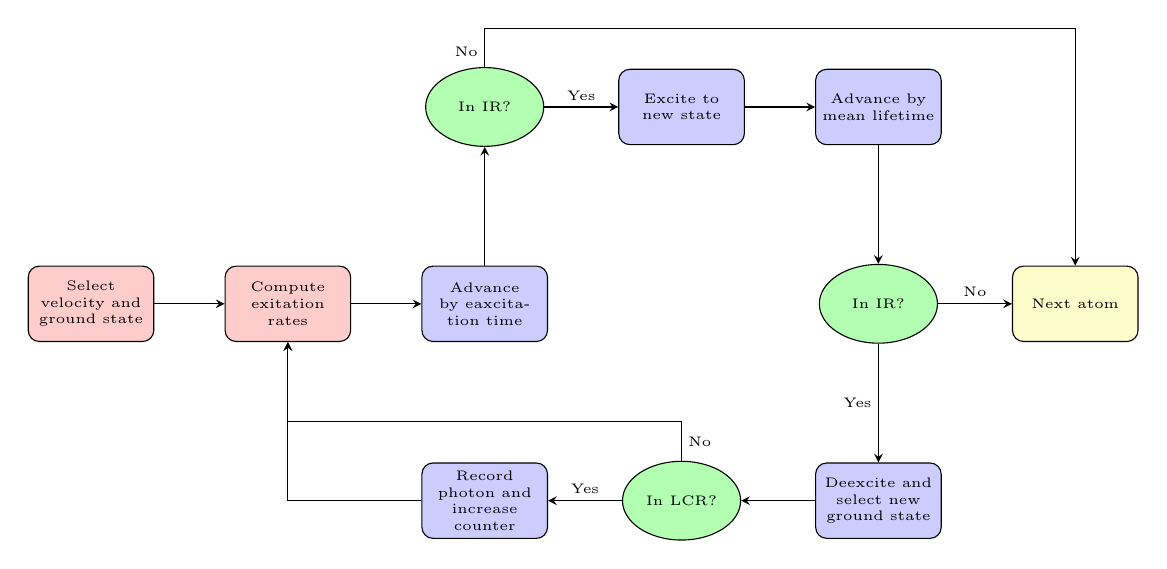
\begin{tikzpicture}[node distance = 2.5cm]
\tiny

\node (props) [prelim] {Select velocity and ground state};
\node (exprobs) [prelim, right of=props] {Compute exitation rates};
\node (Adv_exc) [block, right of=exprobs] {Advance by eaxcitation time};
\node (IR) [decision, above of=Adv_exc] {In IR?};
\node (Exc) [block, right of=IR] {Excite to new state};
\node (Adv_life) [block, right of=Exc] {Advance by mean lifetime};
\node (IR_2) [decision, below of=Adv_life] {In IR?};
\node (Next) [end, right of=IR_2] {Next atom};
\node (deex) [block, below of=IR_2] {Deexcite and select new ground state};
\node (LCR) [decision, left of=deex] {In LCR?};
\node (PHO) [block, left of=LCR] {Record photon and increase counter};
\node[coordinate] (bl1) [above of = IR,yshift=-15mm]{};
\node[coordinate] (bl2) [above of=Next]{};
\node[coordinate] (bl3) [above of=bl2,yshift=-15mm]{};
\node[coordinate] (bl4) [above of = LCR,yshift = -15mm]{};
\node[coordinate] (bl5) [left of =PHO,yshift = 5mm]{};

\draw [arrow] (props)--(exprobs);
\draw [arrow] (exprobs)--(Adv_exc);
\draw [arrow] (Adv_exc)--(IR);
\draw [arrow] (IR) -- node[anchor=south] {Yes} (Exc);
\draw (IR) -- node[anchor=north east,yshift = 1mm] {No} (bl1);
\draw (bl3) -- (bl1);
\draw [arrow] (bl3)--(Next);
\draw [arrow] (Exc)--(Adv_life);
\draw [arrow] (Adv_life) -- (IR_2);
\draw [arrow] (IR_2) -- node[anchor = south] {No} (Next);
\draw [arrow] (IR_2) -- node[anchor = east] {Yes} (deex);
\draw [arrow] (deex) -- (LCR);
\draw [arrow] (LCR) -- node[anchor = south] {Yes} (PHO);
\draw (LCR)-- node[anchor = west] {No} (bl4);
\draw [arrow] (PHO) -| (exprobs);
\draw [arrow] (bl4)-|(exprobs);
\end{tikzpicture}
\caption[Flow chart detailing the steps undertaken by the alternative algorithm to follow the atom as it moves through the IR.]{\small Flow chart detailing the steps undertaken by the algorithm to follow the atom as it moves through the IR. The green ellipses and blue rectangles compose the interaction loop of the simulation, where the atom interacts with the laser and goes through excitation/decay cycles. Finally, the yellow rectangle is the end point of the loop, and occurs when then atom has moved beyond the IR.}
\label{pipeline}
\end{figure}

\label{pip}


\section{Interaction Loop}


Fig. \ref{pipeline} shows each step taken an atom as it passes through the simulation. The red rounded rectangles represent preliminary steps in the simulation, where initial properties are imparted to the atom. The first preliminary step selects a velocity and ground state for the atom. The following step is the calculation of the likelihood of excitation for each allowed transition. This prepares the atom for what can be considered the main loop of the algorithm. Here, the atom and laser interact as the atom traverses the IR. 

The interaction loop is composed of green ellipses and blue rectangles. Two of the three green ellipses represent regular checks to ensure that the atom is still in the IR. If at any point the atom is found to have moved beyond the IR, then the algorithm moves on to the next atom. The third green ellipse is dedicated to checking if a photon released by the atom would be measured by the PMT. The evolution of the state and position of the atom is described by the blue rectangles. 

\subsection{Preliminary Steps}
The first two steps select the initial properties given to the atom, determining how likely the atom is to interact with the laser. The two most important properties are the velocity and the ground state of the atom. Both are chosen through the sampling of their respective probability distributions.

\subsubsection{Velocity Selection}

The velocity of the atom $v_a$ can be decomposed in to two elements: the mean velocity of the beam, $v_{m}$, and the thermal velocity $v_{T}$. 
\begin{equation}
v_a = v_m + v_T
\end{equation}
The mean velocity is determined by the energy of the beam and the mass of the atom, i.e.
\begin{equation}
v_{m} = \sqrt{\frac{2E_b}{m_A}}
\end{equation}
where $E_b$ is the energy of the beam and $m_A$ is the mass of an atom with mass number $A$.

The thermal velocity is selected by sampling the Maxwell-Boltzmann distribution (Eq. \ref{MBD}). This is done using the Box-Muller transform, which samples a uniform distribution twice and converts the results into a sample of a normal distribution. A sample $v_T$, of a Maxwell-Boltzmann distribution
\begin{equation}
v_T = \sigma_{MB} \sqrt{-2\log x_1}\cos (2\pi x_2)
\end{equation}
where $x_1,x_2 \in [0,1]$ are two randomly generated numbers taken from a uniform distribution and $\sigma_{MB}$ is the square root of the variance of the Maxwell-Boltzmann distribution. 

\subsubsection{Ground State Selection}
For an atom with a coupled angular momentum state $F_g$ as the ground state, the electron can occupy any of the $2F_g+1$ projections on the axis of quantization. A particular projection, say $F_i \in [-F_g,-F_g+1,...,F_g-1,F_g]$, has a probability of being occupied that is proportional to $2F_i+1$. Taking the probability space occupied by each projection in to account, the probability that an electron occupies the projection $F_i$, $P(F_i)$, is given by
\begin{equation}
P(F_i) = \frac{2F_i+1}{\sum_j 2F_j+1}
\label{gs_prob}
\end{equation}
Knowing this, the ground state can be chosen through the generation of a random number $x \in [0,1]$ from a uniform distribution. Each projection is given a range of numbers from 0 to 1, proportional to Eq. \ref{gs_prob}. If $x$ falls in the assigned range, then that ground state is chosen. 

\subsubsection{Computation of Excitation Rates}
With the ground state and the velocity of the atom now selected, the probability that a transition will occur can be calculated. For each allowed transition between the chosen ground state $F_g$ and an excited state $F_{e,i}$, the transition rate $\gamma_i$ is given by Eq. \ref{scatt_rate}. Note that the laser frequency $f_l$ must be shifted according to Eq. \ref{dop_shift}.

\subsection{Interaction Loop}
The interaction loop of the algorithm is the place where the atoms undergo several instances of excitation and decay. Also included are regular checks to see in the atom would still be present in the in interaction region, as well as whether or not a released photon would be measured by the light collection system present in the experiment.

\subsubsection{Excitation Time}
Once all the excitation rates have been computed, the atom can now be advanced by the expected time it takes for a transition to occur. This time is called the excitation time, $t_e$, and is given by
\begin{equation}
t_e = \sum_i \frac{1}{\gamma_i}
\end{equation}
After time $t_e$, the atom is advanced a distance $d_e = t_ev_a$. If it is still in the interaction region, then an excited state $F_e$ is chosen by sampling a uniform distribution where each transition is given a region proportional to $1/\gamma_i$, in similar style to the method used to select the ground state. If the atom is no longer in the interaction region after $t_e$, then it is discarded and the algorithm moves on to the next atom.

\subsubsection{Advancing by the Mean Lifetime, Decay and Selection of New Ground State}
Once the excited stated of the atom has been selected, then the atom is advanced a distance $d_l = t_lv_a$ where $t_l$ is the mean lifetime of the excited state. The mean lifetimes of each excited state are computed (according to $\S$ \ref{ALI}) once at the beginning of the simulation, then stored for later use. If the atom is still in the interaction region after having moved $d_l$, then it decays into one of the allowed ground states. If not, then the simulation moves on to the next atom. As with the selection of the excited state, a uniform distribution is sampled, and each ground state $F_{g,i}$ is given a range of values proportional to the inverse of the lifetime of the transition from the excited state, $F_{e}$, to $F_{g,i}$. 

Once a ground state is selected, a photon with energy given by Eq. \ref{HFE} is "released". If the atom is in the light collection region, then this photon is recorded for later analysis. Additionally, a counter that keeps track of the number of photons collected at each beam energy is increased by one. If the atom is not in the LCR, then nothing is recorded, and the excitation-decay process begins again with the computation of excitation rates.

\subsection{Simulation of Complete Run}
In order to simulate a complete experimental run, a chosen number of atoms, say N, are passed in sequence through the above loop. This is done in turn for each beam energy in a list of energies that are selected such that the Doppler shifted laser energies range from the lowest energy to the highest energy transition, with some leeway on either side. This range can be called $E_r$. The graph of photon counts per beam energy is in fact the hyperfine spectrum. Alg. \ref{alg} shows the pseudo-code that is followed for the simulation of a collection of atoms passing through the experiment. Following Alg. \ref{alg} is a list of all the preliminary parameters needed by the simulation in order to compute the necessary quantities presented in this section. 

\vspace{10mm}
\begin{algorithm}[H]
\SetAlgoLined
\KwResult{Simulation of complete hyperfine spectrum}
 Input all preliminary parameters\;
 \For{Beam energy in $E_r$}{
  \For{Each atom}{
   Run \textbf{interaction loop}\;
   Record photon count\;
  }
  Sum photon count into counts per beam energy\;
 }
 Plot photon count at each beam energy\;
 \caption{Pseudo-code for the simulation of a complete hyperfine spectrum.}
 \label{alg}
\end{algorithm}

\vspace{10mm}
The preliminary parameters mentioned in the above pseudo-code refer to all the quantities required to perform a complete simulation of a hyperfine spectrum measured at TRIUMF. A list of these parameters is provided below, for completeness.

\begin{list}{•}{List of Preliminary Parameters and Their Symbols}
\item Isotope mass: $m_A$
\item Ground J-state: $\bf{J}_g$
\item Excited J-state: $\bf{J}_e$
\item Nuclear spin: $\bf{I}$
\item Principal quantum number of ground state: $n_g$
\item Principal quantum number of excited state: $n_e$
\item Magnetic dipole hyperfine coefficient of ground state: $A_g$
\item Magnetic dipole hyperfine coefficient of excited state: $A_e$
\item Electric quadrupole hyperfine coefficient of ground state: $B_g$
\item Electric quadrupole hyperfine coefficient of excited state: $B_e$
\item Beam temperature: $T_b$
\item Laser frequency: $f_l$
\item Laser intensity: $I_l$
\item Fine structure transition energy: $E_{fs}$
\item Number of atoms to simulate per beam energy: $N_a$
\item Distance between CEC and LCR: $d$
\item Length of LCR: $d_{LCR}$
\end{list}

\chapter{Results}
\label{res}
This section presents and examines the results of the modeling outlined in the previous section. $\S$ \ref{Par_stress} shows the effects of changing important input parameters, such as the temperature, on a simulated spectrum of Gallium-69.  

\section{Initial Test}
As a first test, this Fig. \ref{comp} presents a comparison between a measured spectrum of Gallium-69 and a simulated spectrum generated using the parameters given in Tables \ref{hyperfinecoeff} and \ref{othercoeff}.

\begin{figure}[h]
\centering
\includegraphics[width = 0.8\textwidth]{Graphics/Ga-69-vs-sim.png}
\caption[Comparison between a measured spectrum of Gallium-69 and a spectrum simulated.]{\small Comparison between a measured spectrum of Gallium-69 and a spectrum simulated using the parameters given in in Tables \ref{hyperfinecoeff} and \ref{othercoeff}. A reduced $\chi^2$ statistic of 3.167010 is also reported as a measure of accuracy between the simulation and data. A clear difference peak widths of the two spectra can be seen. }
\label{comp}
\end{figure}

\begin{table}[h]
\centering
\begin{tabular}{c c c c}\hline
$A_u$ (MHz)&$A_l$ (MHz)&$B_u$ (MHz)&$B_l$ (MHz)\\ \hline
1070.908128 & 188.512676 & 0 & 68.333737\\ \hline \\
\end{tabular}
\caption[Hyperfine parameters used in the simulation of the spectrum of Gallium-69.]{\small Hyperfine parameters used in the simulation of the spectrum of Gallium-69.\citep{gapap}}
\label{hyperfinecoeff}
\end{table}

\begin{table}[h]
\centering
\begin{tabular}{c c c}\hline
Temperature (K)&Power (mW)&CEC-LCR Dist. (m)\\ \hline
300 & 1.0 & 0.40\\ \hline \\
\end{tabular}
\caption[Other parameters required for the simulation of a hyperfine spectrum.]{\small Other parameters required for the simulation of a hyperfine spectrum. The power and CEC-LCR distance are measured quantities, while the temperature is estimated.}
\label{othercoeff}
\end{table}

A distinct difference in the peak widths between the simulated and measured spectra can be seen in Fig. \ref{comp}, where the simulated spectrum has narrower peaks than the measured spectrum. Since the temperature is merely an estimate based on the cooling methods used to bunch the atoms, it is possible that the estimated temperature is inaccurate. Fig. \ref{chi_temp} shows the reduced $\chi^2$ statistic as a function of the temperature used in the simulation. The estimated temperature of 300 K is lower than the temperature that produces the lowest reduced $\chi^2$ value, occurring at $\sim$910 K.
\begin{figure}[h]
\centering
\includegraphics[width=0.8\textwidth]{Graphics/temp_chi.png}
\caption[Reduced $\chi^2$ statistic as a function of the temperature used in the simulation of a Gallium-69 hyperfine spectrum.]{\small The reduced $\chi^2$ statistic as a function of the temperature used in the simulation of a Gallium-69 hyperfine spectrum. The estimated temperature of 300 K is shown, as well as the temperature at which a minimum in the $\chi^2$ value occurs, $\sim$ 910 K.}
\label{chi_temp}
\end{figure}
\section{Temperature, CEC-LCR Distance and Power}
\label{Par_stress}
In this section, the effects of changing the temperature of the beam, the distance between the CEC and the LCR, and  the laser power  are shown and discussed. 

\subsection{Temperature}
The temperature of the atoms as they interact with the laser is expected to affect the widths of the peaks in the resulting hyperfine spectra. Eq. \ref{temp_width} describes the effects of temperature on the Gaussian contribution to the width of a Voigt profile. Fig \ref{temp_comp} shows the effects of temperature on a simulated spectrum of Gallium-69. As the temperature increases doppler broadening begins to dominate the width of the peaks and the hyperfine structure of the spectrum is diluted. 
\begin{figure}[h!]
\begin{center}
\includegraphics[width = 0.8\textwidth]{Graphics/temp_comparison.png}
\end{center}
\caption[The effects of the temperature on the hyperfine spectrum of Gallium-69.]{\small The effects of the temperature on the hyperfine spectrum of Gallium-69. As the temperature of the atoms increases, the doppler contribution to the width of the peaks increases. At sufficiently high temperatures ($\approx 2.0 \times 10^3$ K), the hyperfine structure of the atom begins to smooth out.}
\label{temp_comp}
\end{figure}

\subsection{CEC-LCR Distance}
Eq.\ref{prob_unchanged} inversely depends on the distance between the CEC and the LCR. The likelihood of an atom reaching the LCR in its original ground state decreases as the CEC-LCR distance increases. Conversely, this likelihood increases as the CEC-LCR distance decreases. Fig \ref{CEC-LCR} shows the effects of changing this distance on a simulated Gallium-69 spectrum. Between 0.1 and 1.0 m, there is no discernible difference between the simulated spectra. As the distance is increased to 2 and then 5 m, optical pumping begins to take effect, with the right-most peak being nearly pumped out at 5 m. 
\begin{figure}[h!]
\begin{center}
\includegraphics[width=0.8\textwidth]{Graphics/dist_comparison.png}
\end{center}
\caption[The effects of changing the CEC-LCR distance on a simulated spectrum of Gallium-69.]{\small The effects of changing the CEC-LCR distance on a simulated spectrum of Gallium-69. As the distance increases, optical pumping begins to have a larger effect. At 5 m, the central peak begins to completely dominate the spectrum at the expense of the smaller peaks near 1.5 and 4 $\times 10^{-3}$+2.9709512 eV.}
\label{CEC-LCR}
\end{figure}

\subsection{Laser Power}
The power of the laser is the most important parameter when simulating the effects of optical pumping on a hyperfine spectrum. This sections first shows the behavior of the model as the power is changed. Figures \ref{power1-40} and \ref{power50-100} show how a simulated spectrum of Gallium-69 changes as the power of the exciting laser is increased from 1.0 to 100 mW. 

\begin{figure}[h!]
\begin{center}
\begin{subfigure}{0.75\textwidth}
\includegraphics[width = \textwidth]{Graphics/Power_comparison(1-40).png}
\caption[The effects of the power of the exciting laser on a simulated Gallium-69 spectrum.]{\small The effects of the power of the exciting laser on a simulated Gallium-69 spectrum are shown above. As the power of the laser is increased, certain transitions become less likely with respect to others, changing the relative intensities of the peaks. }
\label{power1-40}
\end{subfigure}

\begin{subfigure}{0.75\textwidth}
\includegraphics[width = \textwidth]{Graphics/Power_comparison(50-100).png}
\caption[Continuation of Fig \ref{power1-40}]{\small Increasing the power of the laser causes optical pumping to have a greater effect on the resulting spectrum. Peaks corresponding to transitions that have lower likelihoods of reaching the LCR in their original ground states have relative intensities that decrease with respect to the more resilient peaks. }
\label{power50-100}
\end{subfigure}
\end{center}
\end{figure}

\pagebreak
\subsubsection{Rubidium-87}
In a recent experimental run at TRIUMF, a hyperfine spectrum of Rubidium-87 (I = 1.5, $J_e$ = 1.5, $J_g$ = 0.5) was examined as the power of the exciting laser was changed. Below are the results of the run, compared to the spectra predicted by the algorithm described in the previous chapter.

\begin{figure}[h]
    \centering
    \begin{subfigure}[b]{0.49\textwidth}
        \includegraphics[width=\textwidth]{Graphics/100_101.png}
        \caption{}
    \end{subfigure}
    \begin{subfigure}[b]{0.49\textwidth}
        \includegraphics[width=\textwidth]{Graphics/098_099.png}
        \caption{}
        \label{}
    \end{subfigure}
    
  	\begin{subfigure}[b]{0.49\textwidth}
        \includegraphics[width=\textwidth]{Graphics/119_120.png}
        \caption{}
    \end{subfigure}
    \begin{subfigure}[b]{0.49\textwidth}
        \includegraphics[width=\textwidth]{Graphics/096_097.png}
        \caption{}
        \label{}
    \end{subfigure}
    \caption[Comparison between the simulated and measured hyperfine spectra of Rubidium-87 for different laser powers.]{\small Comparison between the simulated (red) and measured (black) hyperfine spectrum of Rubidium-87 for laser power: (a) 4.5 $\mu W$ (b) 8.7 $\mu W$ (c) 12.5 $\mu W$ (d) 18.9 $\mu W$. The lack of data between the two groups of peaks is due to the method of scanning used. To reduce the collection time required, only the regions where peaks were expected were scanned. Also shown are the reduced $\chi^2$ values for each comparison. The simulated spectra tend to exaggerate the effects of optical pumping, exemplified by the predicted height of the left-most peak. In each case, this peak is much lower than the corresponding peak in the measured spectrum. }
    \label{power4-18}
\end{figure}
Fig. \ref{chi_vs_power} shows the performance of the model when compared to the Rubidium-87 spectra. The reduced $\chi^2$ statistic is reported for each Rubidium spectrum and is plotted as a function of the laser power. As a general trend, the model accuracy decreases as the power increases. Examining the comparisons between the predicted and measured spectra of Rubidium-87, a discrepancy between the expected and measured height of the lowest energy peak, located at $\sim$ 0.75e-5+1.58903 eV, is present across all laser powers, indicating that the model overestimates the effects of optical pumping for this transition ($F_e$ = 1 $F_g$ = 0).

\begin{figure}[t!]
	\centering
    \begin{subfigure}[b]{0.49\textwidth}
        \includegraphics[width=\textwidth]{Graphics/107_108.png}
        \caption{}
    \end{subfigure}
    \begin{subfigure}[b]{0.49\textwidth}
        \includegraphics[width=\textwidth]{Graphics/094_095.png}
        \caption{}
        \label{}
    \end{subfigure}

    \begin{subfigure}[b]{0.49\textwidth}
        \includegraphics[width=\textwidth]{Graphics/121_122.png}
        \caption{}
    \end{subfigure}
    \begin{subfigure}[b]{0.49\textwidth}
        \includegraphics[width=\textwidth]{Graphics/111_112.png}
        \caption{}
        \label{}
    \end{subfigure}
    \caption[Continuation of Fig. \ref{power4-18}.]{\small Continuing from Fig. \ref{power4-18}, a comparison between the simulated (red) and measured (black) hyperfine spectrum of Rubidium-87 for laser power: (a) 22.1 $\mu W$ (b) 24.0 $\mu W$ (c) 24.4 $\mu W$ (d) 36.4 $\mu W$. Also shown are the reduced $\chi^2$ values for each comparison. Following the trend shown in the previous spectra, the simulated spectra tend to exaggerate the effects of optical pumping, shown by the discrepancy between the predicted and measured heights of the left-most peak. In each case, this peak is lower than the corresponding peak in the measured spectrum. }
\label{power22-36}
\end{figure}
\pagebreak
\begin{figure}[h]
	\centering
    \begin{subfigure}[b]{0.49\textwidth}
        \includegraphics[width=\textwidth]{Graphics/113_114.png}
        \caption{}
        \label{}
    \end{subfigure}
    \begin{subfigure}[b]{0.49\textwidth}
        \includegraphics[width=\textwidth]{Graphics/115_116.png}
        \caption{}
    \end{subfigure}
    
    \begin{subfigure}[b]{0.49\textwidth}
        \includegraphics[width=\textwidth]{Graphics/117_118.png}
        \caption{}
        \label{}
    \end{subfigure}
    \begin{subfigure}[b]{0.49\textwidth}
        \includegraphics[width=\textwidth]{Graphics/chi-v-power.png}
        \caption{}
        \label{chi_vs_power}
    \end{subfigure}
    \caption[The final set of spectra exploring the effect of the laser power on the hyperfine spectrum on Rubidium-87.]{\small The final set of spectra exploring the effect of the laser power on the hyperfine spectrum on Rubidium-87, compared to the spectra predicted by the method outlined in Chapter \ref {Op_pump} The laser powers are: (a) 39.1 $\mu W$ (b) 50.1 $\mu W$ (c) 108.0 $\mu W$. Also shown are the reduced $\chi^2$ values for each comparison. (d) shows the reduced $\chi^2$ statistic as a function of the power of the exciting laser for the Rubidium-87 experimental run. As the power increases, the model reproduces the spectrum less accurately, as shown by the increase in the value of the $\chi^2$ statistic. }
\label{power39-108}
\end{figure}


\chapter{Conclusion}
\label{conc}
\noindent In this work, a brief introduction to collinear laser spectroscopy at TRIUMF was presented, followed by the theoretical background necessary to understand the hyperfine structure of an atom. Then, a treatment of optical pumping as a modification to the Racah intensities was described and then used to simulate the effects of optical pumping on the measured hyperfine spectra of both Gallium-69 and Rubidium-87. The effects of the beam temperature, the experimental geometry and the power of the exciting laser were explored on a simulated Gallium-69 spectrum. Increasing the temperature caused the peak width to increase, while increasing the distance between the CEC and the LCR affected the relative heights of the hyperfine peaks. Increasing the laser power caused the relative peak heights to change. Continuously increasing the laser power led to the complete domination of a single transition, with the other transitions being \emph{pumped out}. When compared to measured Gallium-69 spectra, there was a discrepancy between the assumed beam temperature (~300 K) and the temperature that produced most accurate simulation (~910 K), possibly caused by an inaccurate estimation of the cooling effects of the RFQ, or a broadening effect caused by the accelerating voltages. When compared Rubidium-87 spectra measured using different laser powers, the simulation consistently underestimated the height of the lowest peak. The discrepancy between the measured and simulated Rubidium-87 spectra seemed to increase with laser power. Given that the simulation was accurate in one case and inaccurate in the other, there is likely some merit in comparing the simulation to different isotopes in future experiments. 


\begin{appendices}
\chapter{Written Code}
\label{code}
\input{code_include/code_include.tex}
\end{appendices}

\bibliography{julienreferences.bib}

\end{document}


 






